


\begin{table}[t]
\centering
\begin{tabular}{rrccc}
\toprule
& & Successful & Failed & Total\\
\midrule
&min &1&1&1\\
\#work item & avg  & 16.68&26.52&19.63\\
& max & 111&109&111\\
\midrule
& min & 1&1&1\\
\#change set & avg  & 26.71&46.27&32.57\\
& max & 227&194&227\\
\midrule
& min & 1&1&1\\
\#Developers & avg  & 19.62&28&22.16\\
& max &64&71&71\\
\bottomrule
\end{tabular}
\caption{Statistics on Jazz data: change sets, work items, 
and developers over successful (227), failed (99) and total builds (328).}
\label{tab:jazzbuildinfo}
\end{table}

\begin{figure}[b]
\centering
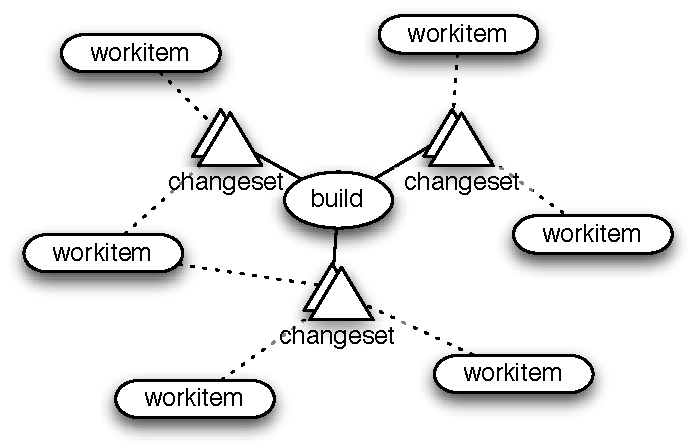
\includegraphics[width=.9\columnwidth]{buildworkitem}
%\vspace{-.3cm}
\caption{Linking work items to builds using change sets.}
\label{fig:buildtowork item}
\end{figure}

\begin{figure}[t]
\centering
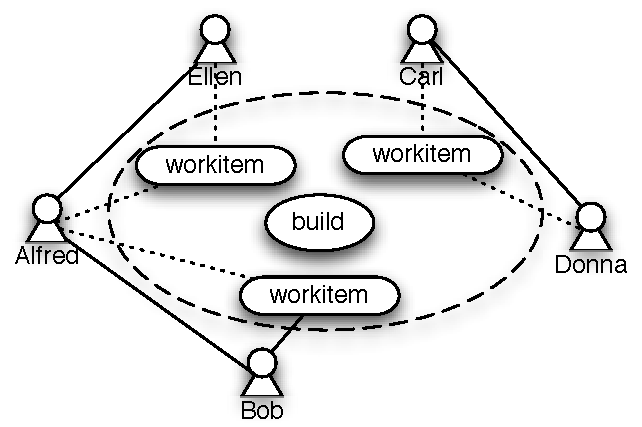
\includegraphics[width=.9\columnwidth]{buildsn}
%\vspace{-.3cm}
\caption{Social network connecting developers through discussions about
work items in a build}
\label{fig:buildsn}
\end{figure}


















\section{Socio-technical coordination\\ and builds in Jazz}
\label{sec:data}
Before we describe our approach to collect data and construct
socio-technical networks in Jazz, we give a brief
description of the Jazz\texttrademark\ team and project. Subsequent,
we explain our approach of mining the project archives to construct
socio-technical networks (Subsections~\ref{subsec:social}
and~\ref{subsec:technical}).

\subsection{Development and Builds in the Jazz Team}
%\subsection{Coordination and integration in Jazz}
The Jazz\tm\ team is a large distributed team and uses the Jazz\tm\ platform for
development. The Jazz\tm\ development involves distributed collaboration over 16
different sites located in the United States, Canada, and Europe. Seven sites are
active in Jazz development and testing. There are 151 active contributors
working in 47 teams at these locations, where developers can belong to multiple
teams. Each team is responsible for developing a subsystem or component of Jazz\tm\.
The team size ranges from 1 to 20 and has an average of 5.7 members. The number
of developers per geographical site ranges from 7 to 24 and is 14.8 in average.

The project uses the \emph{Eclipse Way} development process~\cite{Frost:2007ff}.
It defines six-week iteration cycles, which are separated into planning,
development and stabilization activities. A project management committee
formulates the goals and features for each release at the beginning of the each
iteration, and \emph{work items} represent assignable and traceable tasks for each
team.
Furthermore, the Jazz\texttrademark\ team's development process demands that the developers coordinate using work item discussion. 

The coordination process within
each iteration requires the integration of subsystems developed by individual
Jazz\tm\ teams in a major milestone build of the product.
Each team owns a source code Stream for collaboration and concurrent
implementation of the subsystem. A Stream is the Jazz\tm\ equivalent to a branch of a
source configuration management system, such as Subversion.

A continuous integration process takes place at team-level or project-level. In
frequent intervals, each integration build (referred to a build henceforth)
compiles, packages, and tests the source code of a stream. At the team-level,
contributors commit code changes that are encapsulated in change sets from
their own workspace to the Team Stream. The team integrations build the
subsystem developed by the team. Once a team has a stable version within the Team
Stream, the team publishes the change sets into the Jazz\tm\ Project Integration
Stream. At the project level, the automated
Jazz\tm\ integration builds the subsystems of all teams. 
%The Jazz project-level
%integration takes place \et{nightly}, \et{weekly}, and at the end of each
%iteration -- \et{beta} build.

%%%%%%%%%%%


%We analyze builds created by IBM's Jazz\texttrademark\ development team.
%The Jazz team builds on a regular basis on a nightly and weekly basis.
%Those builds are both on a component and on a project basis.
%
%The Jazz team uses the software they develop the IBM Jazz\texttrademark.
%IBM Jazz\tm\ integrates both source code control and task management.
%Additionally you can also define build schedules as well as general development processes, such as SCRUM.
%
%Thus, the Jazz repository contains all the information from builds over source code changes to tasks, such as bug fixes.
%One advantage of working with he Jazz repository is that links between builds and changes, and changes and tasks are explicit.
%This means we know from the repository which changes contributed to a build and which changes where made to accomplish a task.
%Using this information we can infer which tasks influenced which builds.
%
%The Jazz development team follows the Eclipse Way of development~\cite{Frost:2007ff}.
%The team was between April and July 2008 on a six week development cycle during which a set of features and bug fixes needs to be implemented.
%Instead of extending the cycles when features or bug fixes would take longer to complete they reschedule it for the next cycle.
%
%Another important aspect to their process directly impacts the way they communicate or record their communication.
%Since the Jazz development team is distributed across several sites in North America and Europe they implemented a process that enforces them to record all their communication around any task in the repository.
%This is a best practice implemented by the former Eclipse developer to ensure that people offside do know what's going on and to enable them to contribute.

% some stats about the repository and the team
We mined the Jazz project repository between April and July 2008, and analyzed a
total of 328 builds, out of which 99 were failed and 227 were successful.
Table~\ref{tab:jazzbuildinfo} contains summary statistics describing the Jazz\tm\
repository. We report different aggregations (minimum, average and maximum) of
number of work items, change sets, and developers over all builds. 


%%%%%%%%%%%%%%%%%%%%%%%%%%%%%%%%%%%%%%%%%%%%%%%%%%%%%

%\begin{figure}[t]
%\centering
%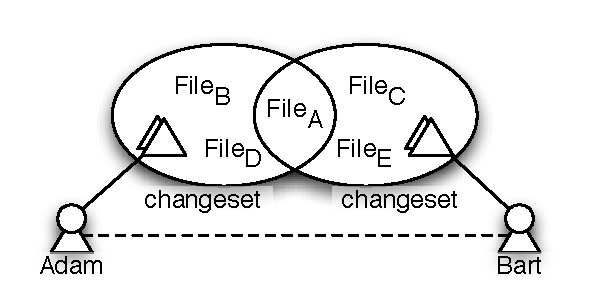
\includegraphics[width=.9\columnwidth]{cochangedfiles}
%%\vspace{-.3cm}
%\caption{Conceptualization of technical relation using co-changed files.}
%\label{fig:technicaldependency}
%\end{figure}

\begin{figure*}[t]
\centering
\subfigure[Identify all change sets related to the social network's build.]{
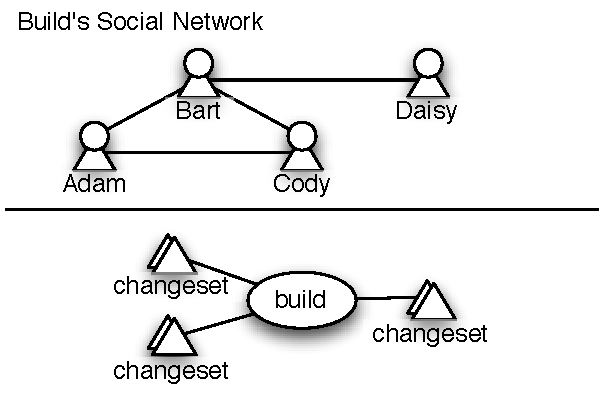
\includegraphics[width=.65\columnwidth]{idcs}
\label{subfig:idcs}
}
\quad
\subfigure[Adding change set owners that are not part of the social network.]{
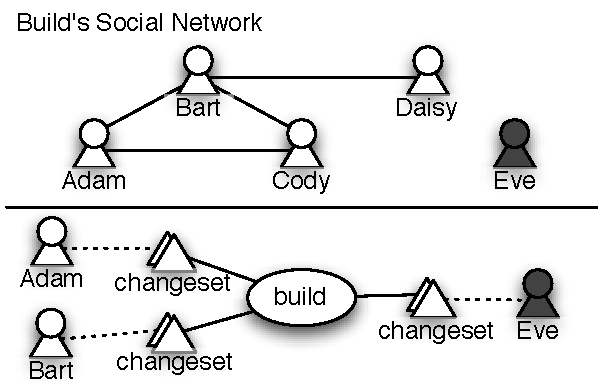
\includegraphics[width=.65\columnwidth]{adduser}
\label{subfig:adduser}
}
\quad
\subfigure[Connect Adam and Bart with a technical edge via the co-changed File$_A$.]{
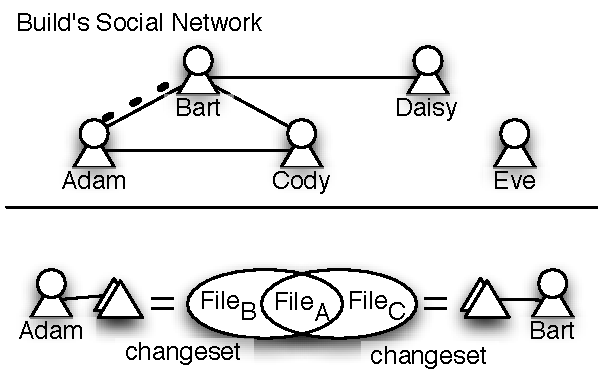
\includegraphics[width=.65\columnwidth]{addedge}
\label{subfig:addedge}
}
%\vspace{-.2cm}
\caption{
Creating a socio-technical network by adding technical dependencies to a build's social-network.}
\label{fig:addtechnicaledge}
\end{figure*}





\subsection{Extracting Social Networks}
\label{subsec:social}
To model the communication between developers for a given build we construct \emph{social networks}. 
We use the information contained in the Jazz\texttrademark\ work items for the construction. 
A \emph{work item} in Jazz\texttrademark\ is the basic unit of work. 
It describes a general task which can be, but is not restricted to, a bug fix or feature request.
Developers coordinate about work on work items by posting comments in a discussion board style which we use as conceptualization of their coordination behavior.
Note that the communication through board discussions is enforced by the team's development process. 


We are interested in constructing a social network for each
build in Jazz\texttrademark. 
To create a social network for a given build we proceed in six steps:

\begin{enumerate}
\item Select the build of interest.
\item Extract change sets that are part of the build.
\item Extract work items linked to the retrieved change sets.
\item Extract developers commenting on a work item before the build's built time.
%\item Retrieve developers that created the retrieved work items.
\item Connect all developers commenting on the same work item.
\end{enumerate}

These steps take us as illustrated in Figure~\ref{fig:buildtowork item}
from a build through a change set to a work item. From the work item we are able to
see who contributed to the work item discussion (Figure~\ref{fig:buildsn}).
These developers become part of the social network and
share a \emph{social edge} if they made a comment on the same work item.
% We use the term \emph{social edge} to describe this connection between two
% developer that commented on the same work item.
Note that all links we use to get from a build to a developer are explicitly contained in
the Jazz\texttrademark\ repository.




\subsection{Constructing Socio-Technical Networks}
\label{subsec:technical}
%\todo{why only change dependencies}
Past research~\cite{nagappan:icse:2005} has shown that dynamic dependencies have the strongest influence on the software quality.
Therefore we use these dynamic dependencies
to construct \emph{socio-technical networks} we use the steps described below
(see Figure~\ref{fig:addtechnicaledge}). We essentially add technical edges to
the build's already constructed social network. In our conceptualization a \emph{technical edge} is a source code
dependency between two developers. A technical dependency between two developers
exists if they changed the same source code file in the build of interest. 

\begin{enumerate}
\item Extract the change sets that are part the build (Figure~\ref{subfig:idcs}).
\item Determine change set owners and add those  that are not already part
of the social network (Figure~\ref{subfig:adduser}).
\item Add a technical edge between change set owners that did change the same file (see Figure~\ref{subfig:addedge}).
\end{enumerate}


We thus call a network that contains both social and technical edges a
\emph{socio-technical network}. The developers in the 
socio-technical network that share both a technical and social edge are said to share
a \emph{socio-technical edge}.









